De manera análoga al caso de espacio libre, se procede a diseñar los adaptadores de cuarto de onda y \texttt{stub}, considerando el valor de carga \ref{ec.z_80_tierra}.

\subsection{Adaptador de cuarto de onda}
\begin{equation*}
	\centering
	Z_a = \sqrt{Z_o \cdot Z_{in}} = \sqrt{ \SI{50}{\ohm} \cdot \SI{1486}{\ohm} } = \SI{272.2}{\ohm}
	\label{ec.z_a_4}
\end{equation*}	

\begin{equation*}
	\centering
	L_a = \frac{\lambda_a}{4} = \frac{ \SI{3.75}{\meter} }{4} = \SI{0.937}{\meter}
	\label{ec.L_a_4}
\end{equation*}


%%% FIGURA PARA CUARTO CON TIERRA
\begin{figure}[H]
	\centering
	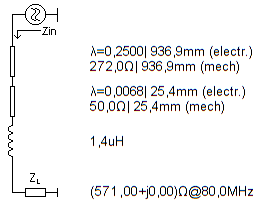
\includegraphics[scale=0.83]{imagenes/smith_4_tierra_esq.png}
	\label{fig.smith_4_tierra_esq}
\end{figure}

\begin{figure}[H]
	\centering
	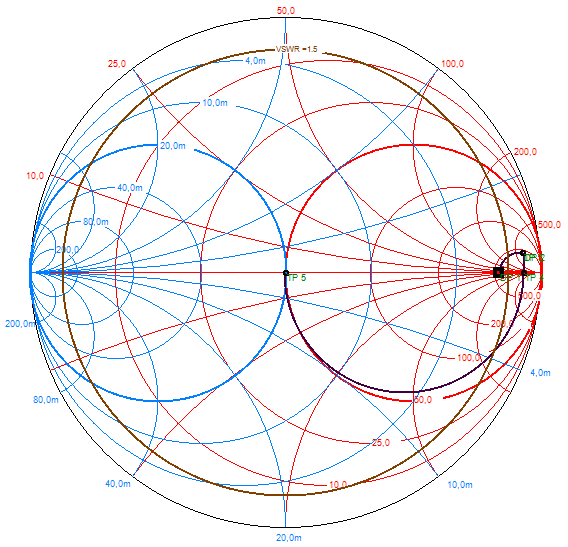
\includegraphics[scale=0.63]{imagenes/smith_4_tierra.png}
	\label{fig.smith_4_tierra}
\end{figure}


\subsection{Stub}
\begin{equation*}
	\centering
	L_s = \num{0.0302}\cdot \lambda = \SI{113.3}{\milli\m}
\end{equation*}

\begin{equation*}
	\centering
	d_s = \num{0.2275}\cdot \lambda = \SI{852.6}{\milli\m}
\end{equation*}


%%%% FIGURA PARA STUB CON TIERRA
\begin{figure}[H]
	\centering
	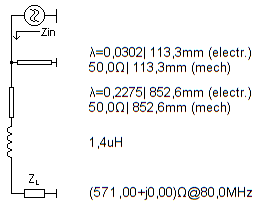
\includegraphics[scale=0.83]{imagenes/smith_stub_tierra_esq.png}
	\label{fig.smith_stub_tierra_esq}
\end{figure}
\begin{figure}[H]
	\centering
	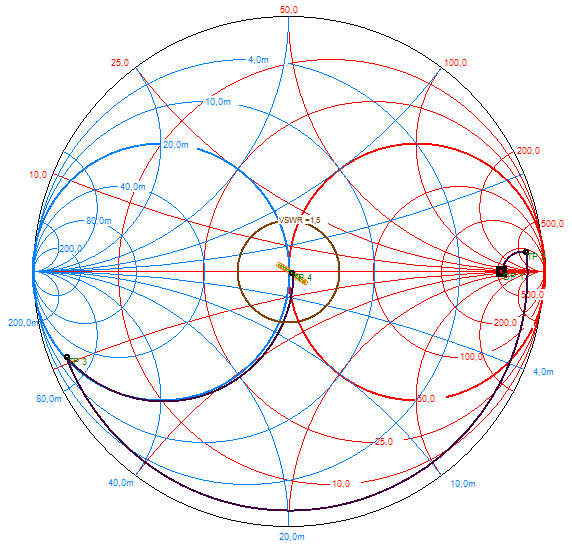
\includegraphics[scale=0.63]{imagenes/smith_stub_tierra.png}
	\label{fig.smith_stub_tierra}
\end{figure}
